\documentclass[11pt,a4paper]{article}
\usepackage[T1]{fontenc}
\usepackage{lmodern}
\usepackage{ngerman}
\usepackage{a4wide}
\usepackage[dvips]{graphicx}

\usepackage[
pdfauthor={ ACE Projekt Team },
pdftitle={ Evaluation Algorithms },
pdfcreator={pdftex},
]{hyperref}

\usepackage{sectsty}
\allsectionsfont{\sffamily}

\usepackage{fancyheadings} 
\pagestyle{fancy} 
\lhead{\textsf{\textbf{ACE} \\ \small{a collaborative editor}}}
\chead{}
\rhead{
\parbox[c]{3cm}{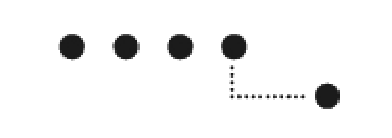
\includegraphics[height=0.875cm,width=3cm]{../../images/logo_BFH.eps}}
\parbox[c]{2.2cm}
{\tiny{\textsf{Berner Fachhochschule \\
Hochschule f�r \\
Technik und Informatik}}}}
\lfoot{}
\cfoot{\textsf{\thepage}}
\rfoot{}
\setlength{\headrulewidth}{0.6pt}
\setlength{\footrulewidth}{0.6pt}
\setlength{\topmargin}{-50pt}
\addtolength{\headheight}{50pt}

\usepackage{colortbl}

\newcommand{\headercol}[2]{\multicolumn{1}{|>{\bfseries\columncolor[gray]{0.82}}p{#1}|}{\textsf{#2}}}
\newcommand{\ace}[0]{\emph{ACE }}



\begin{document}
\setlength{\parindent}{0pt}

\newtheorem{defn}{Definition}

\bibliographystyle{plain}

\begin{titlepage}
\thispagestyle{empty}
  
\includegraphics[height=1.5in]{../images/pix.eps}

  \begin{center}

    {\fontsize{40}{45} \textbf{\textsf{ACE}}} \\
    \textsf{a collaborative editor} \\
        
    \vspace{36pt}
        
    {\huge{\textbf{\textsf{}}}} \\

    \vspace{36pt}

	\textsf{Berne University of Applied Sciences} \\
    \textsf{School of Engineering and Information Technology} \\
    
  \end{center}

  \vfill
  
  \begin{tabular}{ll}
   \hline

   \\

   \multicolumn{1}{>{\bfseries}p{1.5in}}{\textsf{Date:}} &
   \multicolumn{1}{>{}p{4.3in}}{\textsf{08.11.2005}}          \\
   
   \\
   
   \multicolumn{1}{>{\bfseries}p{1.5in}}{\textsf{Version:}}     &   
   \multicolumn{1}{>{}p{4.3in}}{\textsf{0.1}}                 \\

   \\
   
   \multicolumn{1}{>{\bfseries}p{1.5in}}{\textsf{Projectteam:}}                 &
   \multicolumn{1}{>{}p{4.3in}}{\textsf{Mark Bigler (biglm2@hta-bi.bfh.ch)}}  \\
   \multicolumn{1}{>{\bfseries}p{1.5in}}{}                                      &
   \multicolumn{1}{>{}p{4.3in}}{\textsf{Simon Raess (rasss@hta-bi.bfh.ch)}}    \\
   \multicolumn{1}{>{\bfseries}p{1.5in}}{}                                      &
   \multicolumn{1}{>{}p{4.3in}}{\textsf{Lukas Zbinden (zbinl@hta-bi.bfh.ch)}} \\   
   
   \\
   
   \multicolumn{1}{>{\bfseries}p{1.5in}}{\textsf{Receivers:}}                       &
   \multicolumn{1}{>{}p{4.3in}}{\textsf{Jean-Paul Dubois (doj@hta-bi.bfh.ch)}}       \\
   \multicolumn{1}{>{\bfseries}p{1.5in}}{}                                          &
   \multicolumn{1}{>{}p{4.3in}}{\textsf{Claude Fuhrer (frc@hta-bi.bfh.ch)}}       \\

   \\
   
   \multicolumn{1}{>{\bfseries}p{1.5in}}{\textsf{Location:}}               &   
   \multicolumn{1}{>{}p{4.3in}}{\textsf{Subversion Repository}} \\

   \\  
   
   \hline
  \end{tabular}

\end{titlepage}

\newpage

\tableofcontents
\newpage
\listoftables
\listoffigures
\newpage


\section*{Versionskontrolle}

\begin{table}[!h]
 \begin{tabular}{|l|l|l|l|}
  \hline
  \headercol{0.6in}{Version}         & 
  \headercol{0.8in}{Datum}           &
  \headercol{1.2in}{Verantwortlich}  & 
  \headercol{2.8in}{Bemerkungen}     \\
  \hline
  0.1         & 15.03.2005  & rasss           &  Erste Version \\
  \hline
  0.2         & 22.03.2005  & rasss zbinl     &  �berarbeitung \\
  \hline
  0.3         & 30.03.2005  & zbinl           &  Projektspezifisches Vorgehensmodell \\
  \hline
  0.4         & 30.03.2005  & rasss zbinl     &  �berarbeitung Punkte 2, 3 und 4 \\
  \hline
  0.5         & 05.04.2005  & zbinl           &  �berarbeitung Appendix A.1 \\
  \hline
  0.6         & 06.04.2005  & zbinl           &  Anpassungen Punkte 2, 3 und 4 \\
  \hline
  0.7         & 06.04.2005  & Projektteam     &  Review \\
  \hline
  0.8         & 13.04.2005  & Projektteam     &  Letzte Anpassungen \\
  \hline
  1.0         & 13.04.2005  & Projektteam     &  Freigabe \\
  \hline
 \end{tabular}
 \caption{Versionskontrolle}
 \label{Versionskontrolle}
\end{table}

\begin{table}[!h]
 \begin{tabular}{|l|l|l|l|l|}
  \hline
  \headercol{0.9in}{}            & 
  \headercol{0.9in}{Stelle}      & 
  \headercol{0.8in}{Datum}       & 
  \headercol{0.6in}{Visum}       & 
  \headercol{2.0in}{Bemerkungen} \\
  \hline
  \textbf{Freigegeben}   & Projektteam &       &       &             \\
  \hline
  \textbf{Genehmigt}     &             &       &       &             \\
  \hline
 \end{tabular}
 \caption{Pr�fung/Genehmigung}
 \label{Pr�fung/Genehmigung}
\end{table}

\newpage


\section{Introduction}
Real-time cooperative editing systems allow multiple users to view and edit the same document at the same time from multiple sites connected by communication networks. Consistency maintenance is one of the most significant challenges in designing and implementing real-time cooperative editing systems. 

\subsection{Preliminaries}
In this section, some basic concepts and terminologies are introduced. Following Lamport\cite{lamport}, we define a causal (partial) ordering relation on operations in terms of their generation and execution sequences as follows.

\begin{defn}
Causal ordering relation $\rightarrow$: \\
Given two operations $O_{a}$ and $O_{b}$ generated at sites $i$ and $j$, then $O_{a}\rightarrow O_{b}$, iff:
\begin{enumerate}
 \item $i=j$ and the generation of $O_{a}$ $j$, then $O_{a}\rightarrow O_{b}$
 \item or $i \neq $j and the execution of $O_{a}$ at site $j$ happened before the 
       genration of $O_{b}$
 \item or there exists an operation $O_{x}$ such that $O_{a}\rightarrow O_{x}$
       and $O_{x}\rightarrow O_{b}$
\end{enumerate}
\end{defn}

\begin{defn}
Dependent and independent operations: \\
Given any two operations $O_{a}$ and $O_{b}$:
\begin{enumerate}
 \item $O_{b}$ is \emph{dependent} on $O_{a}$ iff $O_{a} \rightarrow O_{b}$
 \item $O_{a}$ and $O_{b}$ are \emph{independent} (or \emph{concurrent}), expressed
       as $O_{a} \Arrowvert O_{b}$ iff neither $O_{a}\rightarrow O_{b}$ nor
       $O_{b}\rightarrow O_{a}$
\end{enumerate}
\end{defn}

Intuitively we can say that two operations are dependant if there is a path from the generation of one message to the generation of another message. So for example in figure \ref{fig:example1} operation $O_{1}$ and $O_{3}$ are dependent, that is $O_{1}\rightarrow O_{3}$. Operation $O_{1}$ and $O_{2}$ are \emph{independent}. 


\subsection{Requirements}
The following requirements have been identified for such systems.

\paragraph{Real-time:} The response to local user actions must be quick, ideally as quick as a single-user editor, and the latency for reflecting remote user actions is low (determined by external communication latency only). 

\paragraph{Distributed:} Cooperating users may reside on different machines connected by communication networks with nondeterministic latency.

\paragraph{Unconstrained:} Multiple users are allowed to concurrently and freely edit any part of the document at any time, in order to facilitate free and natural information flow among multiple users.

The requirements for good responsiveness and for supporting unconstrained collaboration have led researchers to adopt a replicated architecture for the storage of shared documents. The shared documents are replicated at the local storage of each participating site. One of the most challenging problem in designing and implementing real-time cooperative editing systems with a replicated architecture is consistency maintenance of replicated documents. 

To illustrate the challenges researchers are facing, consider a scenario in a cooperative editing system with three cooperating sites, as shown in figure \ref{fig:example1}. Suppose that an operation is executed on the local replica of the shared document immediately after its generation, then broadcast to remote sites and executed there in its \emph{original form} upon its arrival.


\subsection{Three inconsistency problems}
Three different inconsistency problems have been identified by {Sun et. al}\cite{sun:achieving}.

\begin{figure}
 \centering
 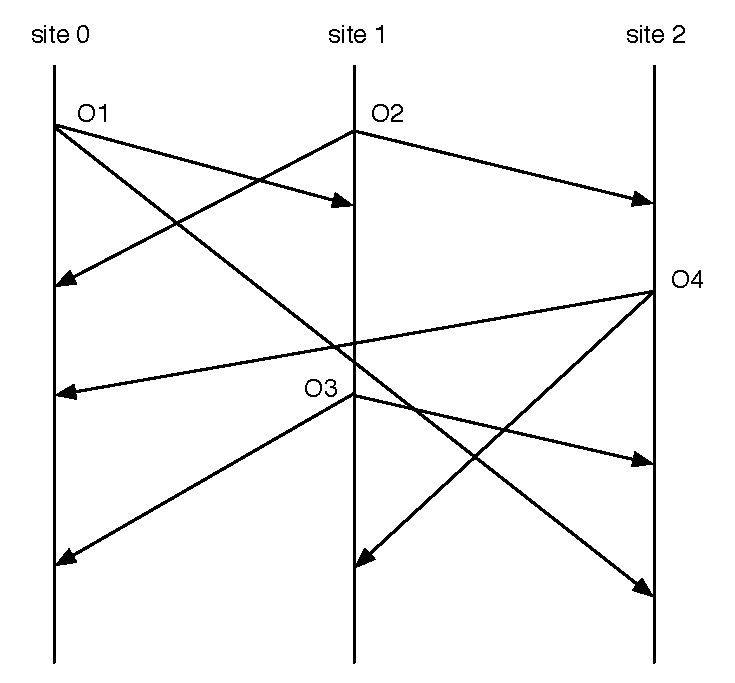
\includegraphics[width=4.68in,height=4.33in]{../../images/example1.eps}
 \caption{A scenarion of a real-time cooperative editing session}
 \label{fig:example1}
\end{figure}

\paragraph{Divergence:}
Operations may arrive and be executed at different sites in different orders, resulting in different final results. As shown in figure \ref{fig:example1}, the four operations in this scenario are execute in the following orders: $O_{1}$, $O_{2}$, $O_{4}$ and $O_{3}$ at site 0; $O_{2}$, $O_{1}$, $O_{3}$ and $O_{4}$ at site 1; and $O_{2}$, $O_{4}$, $O_{3}$ and $O_{1}$ at site 2. Unless operations are commutative, which is generally not the case, final editing results will diverge. The divergence problem can be solved by any serialization protocol, which ensures the final result is the same as if all operations were executed in the same total order at all sites.

\paragraph{Causality violation:}
Due to the nondeterministic communication latency, operations may arrive and be executed out of their natural cause-effect order. As shown in figure \ref{fig:example1}, operation $O_{3}$ is generated after the arrival of $O_{1}$ at site 1, the editing effect of $O_{1}$ on the shared document has been seen by the user 1 at the time $O_{3}$ is generated. Therefore, $O_{3}$ may be \emph{dependent} on $O_{1}$. However, since $O_{3}$ arrives and is executed before $O_{1}$ at site 2, confusion may occure to the system as well as to the user at site 2. For example, if $O_{1}$ is to insert a string into a shared document, and $O_{3}$ is to delete some characters in the string inserted by $O_{1}$, then the execution of $O_{3}$ before $O_{1}$ at site 2 will result in $O_{3}$ referring to a nonexistent context. 

\paragraph{Intention violation:}
Due to concurrent generation of operations, the \emph{actual effect} of an operation at the time of its execution may be different from the \emph{intended effect} of this operation at the time of its generation. As shown in figure \ref{fig:example1}, operation $O_{1}$ is generated at site 0 without any knowledge of $O_{2}$ generated at site 1, so $O_{1}$ is \emph{independent} of $O_{2}$, and vice versa. At site 0, $O_{2}$ is executed on a document state which has been changed by the preceding execution of $O_{1}$. Therefore, the subsequent execution of $O_{2}$ may refer to an incorrect position in the new document state, resulting in an editing effect which is different from the \emph{intention} of $O_{2}$. 

For example, assume the shared document initially contains the following sequence of characters: "'ABCDE"'. Suppose $O_{1}=Insert["'12"',1]$, which intends to insert string "'12"' at position 1, i.e. between "'A"' and "'BCDE"'; and $O_{2}=Delete[2,2]$, which intends to delete the two characters starting from position 2, i.e. "'CD"'. After the execution of these two operations, the \emph{intention-preserved} result (at all sites) should be: "'A12BE"'. However, the actual result at site 0, obtained by executing $O_{1}$ followed by executing $O_{2}$, would be: "'A1CDE"', which apparently violates the intention of $O_{1}$ since the character "'2"', which was intented to be inserted, is missing in the final text, and violates the intention of $O_{2}$ since characters "'CD"', which were intended to be deleted, are still present in the final text.

Even if a serialization-based protocol was used to ensure that all sites execute $O_{1}$ and $O_{2}$ in the same order to get an identical result "'A1CDE"', but this identical result is still inconsistent with the intentions of both $O_{1}$ and $O_{2}$.


\subsection{Operational Transformations}
{Ellis and Gibbs}~\cite{ellis} proposed a new kind of algorithms, called \emph{Operational Transformations} (OT).  These kind of algorithms transform operations, or more specifically their index, to incorporate independent operations.

\subsection{Transformation Properties}
It was shown in \cite{ressel:adopted} that transformation functions must satisfy two conditions, called TP1 and TP2.

\paragraph{Transformation Property 1:}
The transformation property 1 ensures that the effect of executing $O_{1}$ followed by the transformed request $O_{2}$ is the same as executing request $O_{2}$ followed by the transformed request $O_{1}$. 

\begin{defn}
Transformation Property 1 $ O_{1} O'_{2} \equiv O_{2} O'_{1} $
\end{defn}

\paragraph{Transformation Property 2:}
Transformation property 1 is a necessary and sufficient condition to ensure that the groupware system with two users is correct. When there are more than two users, the situation is more complex. An operation can be transformed along different, albeit equivalent paths, not necessarily yielding the same result. In the simplest case, an operation can be transformed along the two paths of a simple transformation step. Operation $O_{1}$ may be transformed first with respect to $O_{2}$ and then to $O'_{3}$ yielding $IT(IT(O_{1},O_{2}),O'_{3})$, or it may be transformed first with respect to $O_{3}$ and then to $O'_{2}$ yielding $IT(IT(O_{1},O_{2}),O'_{2})$. Note that different sites might choose different paths for $O_{1}$ to be transformed. So we have to make sure that both paths lead to the same resulting operation:

\begin{defn}
Transformation Property 2: 
$IT(IT(O_{1},O_{2}),O'_{3})$=$IT(IT(O_{1},O_{2}),O'_{2})$
\end{defn}


\section{History}
{Ellis and Gibbs}~\cite{ellis} were the first to propose an \emph{Operational Transformation} algorithm in 1989. The algorithm is called \emph{dOPT} and is implemented in the \emph{Grove} system. Soon however a flaw was discovered in the original \emph{dOPT} algorithm (by Cormack\cite{cormack}). The scenario where \emph{dOPT} failed is called the \emph{dOPT} puzzle. Ressel\cite{ressel:adopted} proposed a new algorithm \emph{adOPTed} in 1996 that solved the original \emph{dOPT} puzzle. {Sun et. al}\cite{sun:achieving} proposed a new algorithm called \emph{GOT} that similarly to \emph{adOPTed} solved the \emph{dOPT} puzzle. {Sun et. al}\cite{sun:reversible} developed some transformation functions for string-wise operations.

Later research groups\cite{imine:development}\cite{imine:achieving} proved the transformation functions of both Ressel\cite{ressel:adopted} and Sun\cite{sun:achieving} to fail to hold TP2 in certain situations. They proposed new transformation functions they developed using a theorem prover. 

Proving the transformation property 1 (TP1) seems to be rather straightforward. However, proving that a given transformation function holds TP2 appears to be difficult. There are over 100 cases that have to be analyzed (according to {Imine et. al}\cite{imine:achieving}). Imine et. al shows that many proposed transformation functions do not hold TP2. 

Recently, two different ways have been taken to deal with the TP2 problem. One kind of algorithms try to avoid the need to comply with TP2 altogether (SOCT2\cite{},GOT\cite{},SOCT3/4\cite{soct34},TIBOT\cite{tibot}). Other research groups try to correct the problems in the original transformation functions of GOTO\cite{} and adOPTed\cite{ressel:adopted}. 


\section{Algorithms}
In this section we give an overview of all the \emph{Operational Transformation} algorithms we have found so far.

\subsection{dOPT}
\emph{dOPT} is the original operational transformation algorithm developed by {Ellis and Gibbs}\cite{ellis}. It was soon discovered that in some situations the document replicas did not converge. This situation is known as the \emph{dOPT} puzzle.

\subsection{adOPTed}

\subsection{GOT}

\subsection{GOTO}

\subsection{SDT}

\subsection{SOCT2}

\subsection{SOCT3}

\subsection{SOCT4}

\subsection{TIBOT}


\bibliography{ace}

\end{document}



























